\documentclass[12pt]{article}
\usepackage[utf8]{inputenc}
\usepackage{graphicx}
\usepackage{listings}
\usepackage{amsmath}
\usepackage{tensor}
\usepackage{subfigure}
\usepackage{float}
\usepackage{natbib}
\usepackage{url}
%Include packages to have python(or other prog. languages) scripts included in the pdf-file without broken lines
\usepackage{color}
\definecolor{codegreen}{rgb}{0,0.6,0}
\definecolor{codegray}{rgb}{0.5,0.5,0.5}
\definecolor{codepurple}{rgb}{0.58,0,0.82}
\definecolor{backcolour}{rgb}{0.95,0.95,0.92}
\lstdefinestyle{mystyle}{
    backgroundcolor=\color{backcolour},
    commentstyle=\color{codegreen},
    keywordstyle=\color{magenta},
    numberstyle=\tiny\color{codegray},
    stringstyle=\color{codepurple},
    basicstyle=\footnotesize,
    breakatwhitespace=false,
    breaklines=true,
    captionpos=b,
    keepspaces=true,
    numbers=left,
    numbersep=5pt,
    showspaces=false,
    showstringspaces=false,
    showtabs=false,
tabsize=2}
\lstset{style=mystyle}
%Making vectors bold instead of putting arrow on it
\renewcommand{\vec}[1]{\mathbf{#1}}

\begin{document}

\begin{titlepage}

\newcommand{\HRule}{\rule{\linewidth}{0.5mm}}
\center

\textsc{\LARGE University of Oslo}\\[1.5cm]
\textsc{\Large FYS4150}\\[0.5cm]
\textsc{\large Kristine Moseid, Helene Aune og Helle Bakke}\\[0.5cm]

\begin{minipage}{0.4\textwidth}
\end{minipage}\\[1cm]

\HRule \\[0.4cm]
{ \huge \bfseries Introduction to numerical projects}\\[0.4cm]
\HRule \\[1.5cm]

\begin{minipage}{0.4\textwidth}
\end{minipage}\\[8cm]


{\large \today}\\[3cm]
\vfill

\end{titlepage}

\newpage
\tableofcontents

\newpage

\addcontentsline{toc}{section}{Summary}
\subsubsection*{Summary}

\begin{itemize}
\item Tease the reader
\item Write last
\end{itemize}

\addcontentsline{toc}{section}{Introduction}
\subsubsection*{Introduction}

\begin{itemize}
\item Motivate the reader
\item What have we done
\item Structure of report
\end{itemize}

\noindent The aim of this project is to solve the one-dimensional Poisson equation with Dirichlet boundary conditions by rewriting it as a set of linear equations. We will be solving the equation
\begin{align*}
-u^{\prime \prime}(x) = f(x), \quad x \in (0,1), \quad  u(0) = u(1) = 0
\end{align*}
where we define the discretized approximation to $u$ as $v_i$ with grid point $x_i = ih$ in the interval from $x_0$ to $x_{n+1} = 1$, and the step length as $h = 1/(n+1)$.


\addcontentsline{toc}{section}{Methods}
\subsubsection*{Methods}

\begin{itemize}
\item Describe methods and algorithms
\item Explain
\item Calculations to demonstrate the code, verify results(benchmarks)
\end{itemize}

\noindent With the bounadry condition $v_0 = v_{n+1} = 0$, the approximation of the second derivative of $u$ was written as
\begin{align*}
- \frac{v_{i+1} + v_{i-1} - 2v_i}{h^2} &= f_i, \quad i = 1,...,n
\end{align*}
where $f_i = f(x)$. We then rewrote the equation as a linear set of equations:
\begin{align*}
- (v_{i+1} + v_{i-1} - 2v_i) &= h^2f_i \\
\intertext{We solved this equation for a few values of $i$. We also set $h^2f_i = d_i$.}
\intertext{$i = 1$:}
- (v_{1+1} + v_{1-1} - 2v_1) &= d_1 \\
- (v_2 + v_0 - 2v_1) &= d_1 \\
- v_2 - 0 + 2v_1 &= d_1
\intertext{$i = 2$:}
- (v_{2+1} + v_{2-1} - 2v_2) &= d_2 \\
- v_3 - v_1 + 2v_2) &= d_2
\intertext{$i = 3$:}
- (v_{3+1} + v_{3-1} - 2v_3) &= d_3 \\
- v_4 - v_2 + 2v_3) &= d_3
\intertext{We saw that this could be written as a linear set of equations $\vec{A} \vec{v} = \vec{d}$,}
 \left(\begin{array}{cccccc}
 	2& -1& 0 &\dots   & \dots &0 \\
     -1 & 2 & -1 &0 &\dots &\dots \\
     0&-1 &2 & -1 & 0 & \dots \\
     & \dots   & \dots &\dots   &\dots & \dots \\
     0&\dots   &  &-1 &2& -1 \\
     0&\dots    &  & 0  &-1 & 2 \\
     \end{array} \right)
\left(\begin{array}{c}
	v_1 \\
	v_2 \\
	v_3 \\
	\dots \\
	v_{n-1} \\
	v_n \\
	\end{array} \right) =
\left(\begin{array}{c}
	d_1 \\
	d_2 \\
	d_3 \\
	\dots \\
	d_{n-1} \\
	d_n \\
	\end{array} \right)
\end{align*}
\\
\\
%%%%%%%%%%%%%%EXERCISE B%%%%%%%%%%%%%%%%%%%%%%%%%
\\
\newcommand{\RNum}[1]{\uppercase\expandafter{\romannumeral #1\relax}}
The following tridiagonal matrix is written on the general form, For simplicity, lets make n = 4. Note the rownumbers in matrix $\vec{A}$ are called $\RNum{1}$, $\RNum{2}$, $\RNum{3}$ and $\RNum{4}$, respectively. \\
\\
 \left(\begin{array}{cccc}
 	{b_1} &{c_1}&0    &0     \\
    {a_2} &{b_2}&{c_2}&0     \\
     0    &{a_3}&{b_3}&{c_3} \\
     0    &0    &{a_4}&{b_4} \\
     \end{array} \right)
\left(\begin{array}{c}
	v_1 \\
	v_2 \\
	v_3 \\
	v_4 \\
	\end{array} \right) =
\left(\begin{array}{c}
	d_1 \\
	d_2 \\
	d_3 \\
    d_4 \\
	\end{array} \right)

\noindent We used Gaussian elimination, also known as the tridiagonal matrix algorithm \citep{WikiT} to solve the above system. We first decomposed $\vec{A}$ and used forward substitution so that $a_2$, $a_3$ and $a_4$ equals zero. We gave the decomposed row a new name.\\
\noindent We were already happy with $\RNum{1}$, as it had no $a$, moving on we got \\
\begin{align*}
\widetilde{\RNum{2}} = \RNum{2} - \RNum{1}  k_1 = (0, \ \tilde{b_2}, \ c_2, \ 0)     \\
k_1 = \frac{a_2}{b_1}, \ \ \ \tilde{b_2} = b_2 - \frac{a_2 c_1}{b_1} \\
\widetilde{\RNum{3}} = \RNum{3} - \widetilde{\RNum{2}}  k_2 = (0, \ 0 \ \tilde{b_3}, \ c_3) \\
k_2 = \frac{a_3}{\tilde{b_2}}, \ \ \ \tilde{b_3} = b_3 - \frac{a_3 c_2}{\tilde{b_2}}\\
\end{align*}
After doing this for a couple more rows one can clearly see that the algorithm for $k_i$ and $\tilde{b_i}$ can be describes as
\begin{align*}
    k_i = \frac{a_{i+1}}{b_i}, \ \ \ \tilde{b_i} = b_i - \frac{a_i c_{i-1}}{\tilde{b_i}} \\
\end{align*}
\noindent Our newly forward substituted (and simplified) matrix now looks like this \\
\\
 \left(\begin{array}{cccc}
 	{b_1} &{c_1}&0    &0        \\
    0 &{\tilde{b_2}&{c_2}&0     \\
     0    &0&\tilde{b_3}&{c_3}  \\
     0    &0    &0&\tilde{b_4}  \\
     \end{array} \right)
\left(\begin{array}{c}
	v_1 \\
	v_2 \\
	v_3 \\
	v_4 \\
	\end{array} \right) =
\left(\begin{array}{c}
	d_1 \\
	\tilde{d_2} \\
	\tilde{d_3} \\
    \tilde{d_4} \\
	\end{array} \right)

\noindent If we write these matrices out as linear equations, we can solve them for $v$ and find the corresponding algorithm, starting with the bottommost row. \\
\begin{align*}
    \RNum{4}: \tilde{b_4}v_4 = \tilde{d_4} \\
    \RNum{3}: \tilde{b_3}v_3 + c_3 v_4 = \tilde{d_3} \\
    \RNum{2}: \tilde{b_2}v_2 + c_2 v_3 = \tilde{d_2} \\
    \rightarrow v_i = \frac{\tilde{d_i} - c_i v_{i+1}}{\tilde{b_i}}\\
\end{align*}
\\
\noindent Finally, our backwards substitution gives, \\
\begin{align*}
    \tilde{d_2} = \widetilde{\RNum{2}} $\bf{v}$ = (\RNum{2} - \RNum{1}  k_1) $\bf{v}$ = \RNum{2} $\bf{v}$ - \RNum{1} k_1 $\bf{v}$ = d_2 - d_1 k_1 \\
    \tilde{d_3} = \widetilde{\RNum{3}} $\bf{v}$ = (\RNum{3} - \RNum{2}  k_2) $\bf{v}$ = \RNum{3} $\bf{v}$ - \RNum{2} k_2 $\bf{v}$ = d_3 - d_2 k_2 \\
    \rightarrow \tilde{d_i} = d_i - d_{i-1} k_{i-1}
\end{align*}

and we now have our four algorithms to be implemented into our code.\\

%%%%%%%%%%%%%%%%%%%%%METHOD END B%%%%%%%%%%%%%%%%%

\addcontentsline{toc}{section}{Results}
\subsubsection*{Results}

\begin{itemize}
\item Present results
\item Critical discussion
\item Put code etc. on GitHub and explain to reader where they can find it
\item Explanatory figures with captions, labels etc.
\end{itemize}


%%%%%% B %%%%%%%%%%%

\noindent FLOPS is an acronym for floating point operations per second \citep{WikiF}, and is a useful tool to measure computer perfomance. \\
The following table shows the variable names from our general algorithm with their corresponding FLOPS. $\tilde{b_i}$ is a special case as the relation $\frac{c_{i-1}}{b_{i-1}}$ will only need to be computed once. Therefore the amount of FLOPS will be 3 the first time $b_i$ is calculated, but 2 thereafter. \\


\begin{center}
  \begin{tabular}{ l | c }
    &FLOPS \\ \hline
    $\tilde{b_i}$ & 3 (2) \\
    $k_i$& 1 \\
    $v_i$ & 3 \\
    $\tilde{d_i}$ & 2
  \end{tabular}
\end{center}
\\
\noindent Figure \ref{fig:1b} shows how the general tridiagonal matrix algorithm for three different $n$'s compare to the closed form solution. There is a total of four curves in this Figure, with the one for n = 10 (green) giving, as expected, the biggest difference. \\
\noindent The latter three curves are harder to distinguish, so Figure \ref{fig:1bz} shows a zoomed version of Figure \ref{fig:1b}. Here one can see that the larger $n$ value gives the closest result to the closed form solution.
%%%SLITER MED AA FAA BEGGE FIGURENE TIL AA GJORE SOM JEG VIL
\begin{center}
    \begin{figure}[h!]
    %\centering
        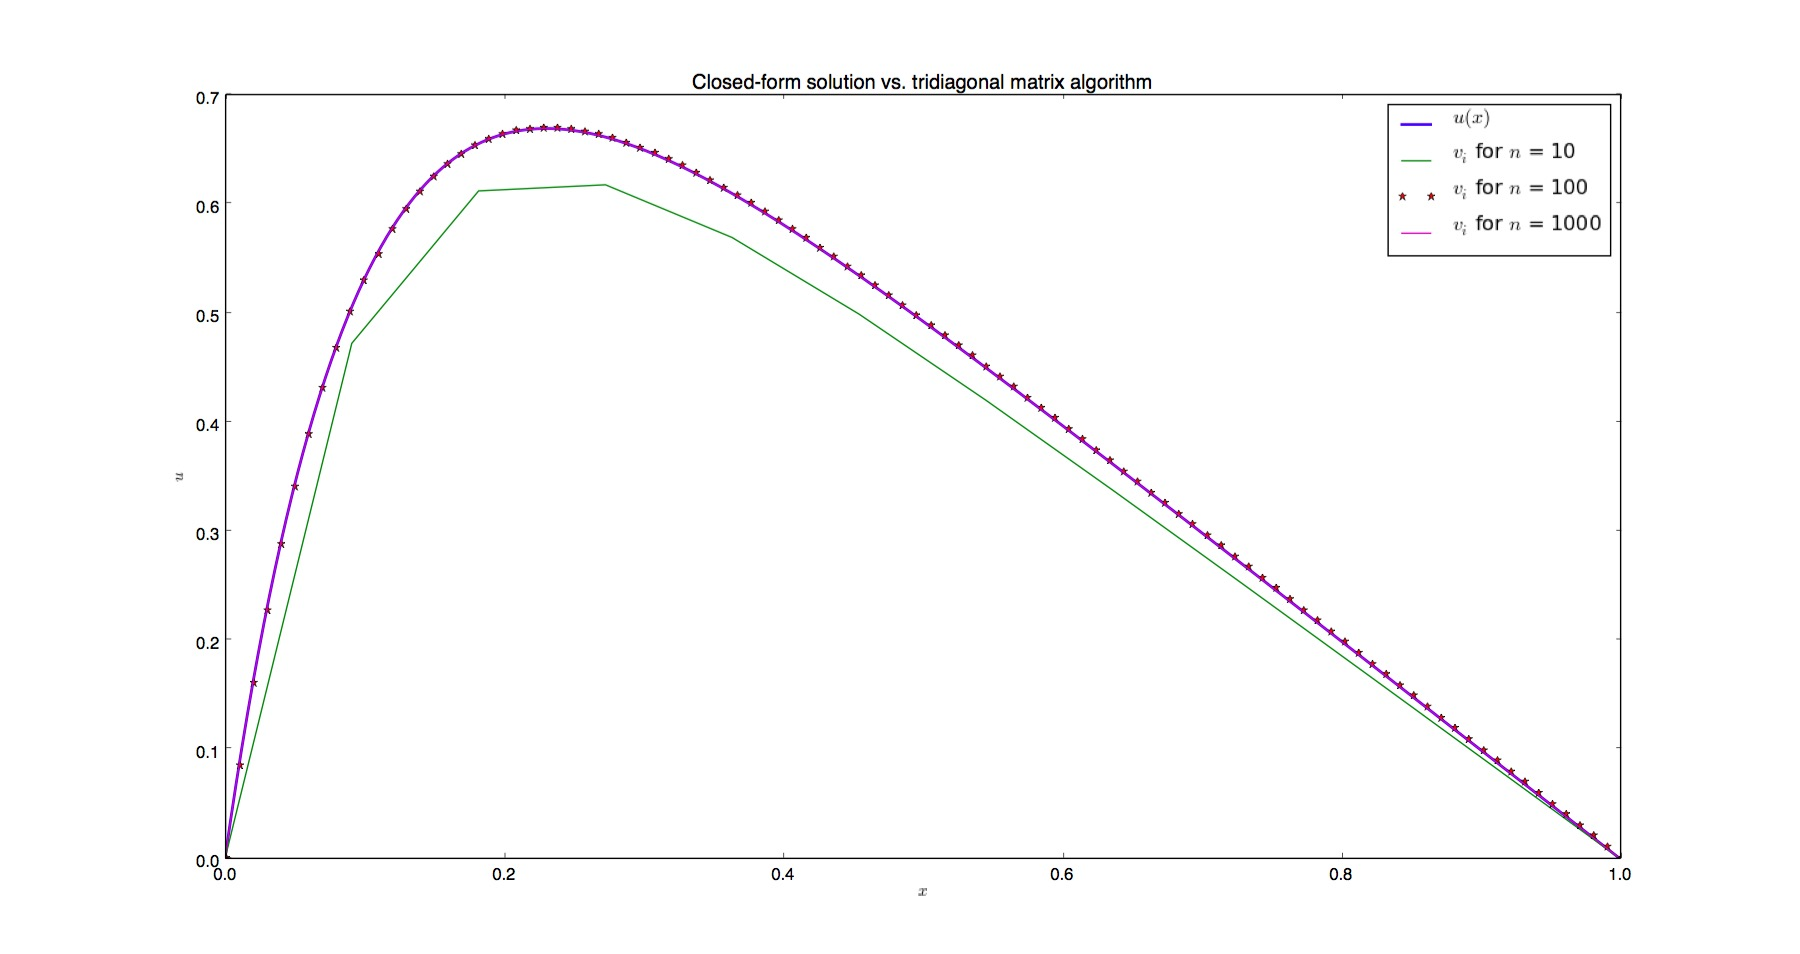
\includegraphics[width=1.4\textwidth]{figure_1b.png}
        \caption{Closed form solution(blue) versus the     tridiagonal matrix algorithm for n = 10     (green), n = 100 (red stars), and n = 1000 (red line). }
        \label{fig:1b}
    \end{figure}
\end{center}

\begin{center}
    \begin{figure}[h!]
    %\centering
        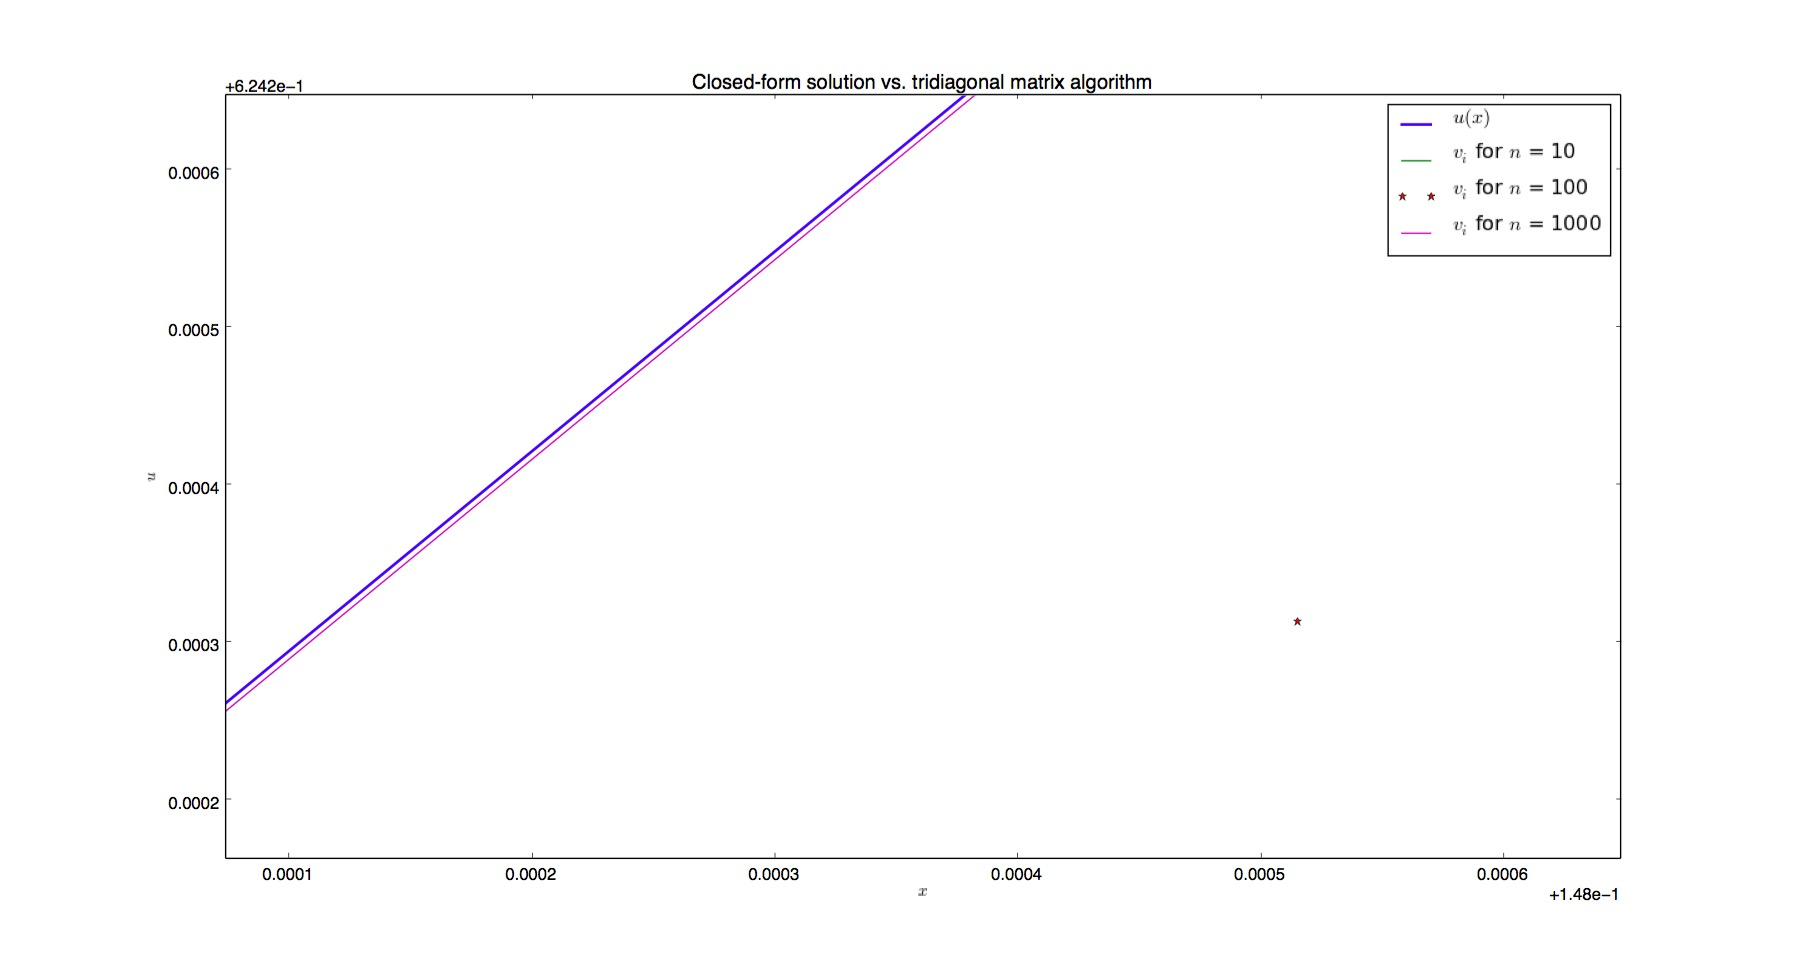
\includegraphics[width=1.4\textwidth]{figure_1b_zoom.png}
        \caption{Closed form solution(blue) versus the     tridiagonal matrix algorithm for n = 100 (red star), and n = 1000 (red line). }
        \label{fig:1bz}
    \end{figure}
\end{center}
%%%% RESULT END B %%%%%

%%%%%%%%%%%%% TABLE FOR D %%%%%%%%%
\begin{center}
  \begin{tabular}{ l | c | c | c | c | c | c | r}
  n & 10 &$10^2$ &$10^3$ &$10^4$& $10^5$&$10^6$&$10^7$\\ \hline
    Error &&&&&&& \\
  \end{tabular}
\end{center}

%%%%% TABLE FOR E %%%
\begin{center}
  \begin{tabular}{ l | c | r }
    n & Tridiagonal method & LU method \\ \hline
    10 & 4.0e-6 & 3.0e-5 \\
    100 & 7.0e-6 & 1.0e-3 \\
    1000 & 5.7e-5& 8.8e-2 \\
  \end{tabular}
\end{center}
%%%%%%%%%%%%%
\addcontentsline{toc}{section}{Conclusion}
\subsubsection*{Conclusion}

\begin{itemize}
\item Main findings
\item Perspectives on improvement and future work
\end{itemize}

\addcontentsline{toc}{section}{Appendix}
\subsubsection*{Appendix}

\begin{itemize}
\item Additional calulations
\item Selected calulations with comments
\item Code, if necessary
\item Appendix can be pushed to GitHub!
\end{itemize}

\addcontentsline{toc}{section}{References}
\subsubsection*{References}

\begin{itemize}
\item Reference to material we based our work on(lecture notes etc.)
\item Find scientific articles, books etc.
\item BibTex - extract references online
\end{itemize}



\bibliographystyle{unsrtnat}
\bibliography{project1}


\end{document}
